% Metódy inžinierskej práce

\documentclass[10pt,twoside,slovak,a4paper]{article}

\usepackage[slovak]{babel}
\usepackage[IL2]{fontenc}
\usepackage[utf8]{inputenc}
\usepackage{graphicx}
\usepackage{url}
\usepackage{hyperref}

\usepackage{cite}

\pagestyle{headings}

\title{Porovnávacia analýza výkonnosti a odolnosti vzorov komunikácie mikroservisov (gRPC, REST, NATS, Kafka) pri sieťových degradáciách\thanks{Semestrálny projekt v predmete Metódy inžinierskej práce, ak. rok 2026/27, vedenie: Meno Priezvisko}}

\author{
    \begin{minipage}{0.45\textwidth}
        \centering
        Ruslan Honcharov\\[2pt]
        {\small \texttt{xhoncharov@stuba.sk}}
    \end{minipage}
    \begin{minipage}{0.45\textwidth}
        \centering
        Mykhailo Hoi\\[2pt]
        {\small \texttt{xhoi@is.stuba.sk}}
    \end{minipage}
    \\[12pt]
    \begin{minipage}{0.45\textwidth}
        \centering
        Hnatiuk Volodymyr\\[2pt]
        {\small \texttt{xhnatiuk@stuba.sk}}
    \end{minipage}
    \begin{minipage}{0.45\textwidth}
        \centering
        Andrii Gladushka\\[2pt]
        {\small \texttt{xgladushka@stuba.sk}}
    \end{minipage}
    \\[14pt]
    {\small Slovenská technická univerzita v Bratislave}\\
    {\small Fakulta informatiky a informačných technológií}
}

\date{\small 4. október 2026}

\begin{document}

\maketitle

\begin{abstract}
Tento projekt sa zaoberá empirickým výskumom a porovnávacou analýzou výkonnosti a spoľahlivosti rôznych komunikačných paradigmát v mikroservisnej architektúre (HTTP/REST, gRPC, NATS JetStream, Apache Kafka). Hlavným cieľom je preskúmať správanie systému pri simulovaných sieťových poruchách (zvýšená latencia, strata paketov, sieťový split) a vyhodnotiť efektivitu vzorov odolnosti (Circuit Breaker, Retries s exponenciálnym odstupom, Rate Limiting). Výstupom práce je testovací stojan pre Chaos Engineering a matica odporúčaní pre návrh odolných distribuovaných systémov s ohľadom na metriky priepustnosti (RPS), latencie (P95/P99) a chybovosti.
\end{abstract}

\section{Úvod}

V modernom vývoji softvéru sa architektúra mikroservisov stala štandardom pre budovanie škálovateľných a flexibilných systémov~\cite{Newman2021}. Na rozdiel od monolitických aplikácií, kde komunikácia prebieha v rámci jedného pamäťového priestoru, mikroservisy intenzívne využívajú počítačovú sieť. Sieť však z hľadiska distribuovaných systémov neponúka absolútnu spoľabilivosť — bežne dochádza ku kolísaniu latencie, strate paketov alebo dočasným výpadkom uzlov.

Pokiaľ nie je komunikačná vrstva správne navrhnutá, lokálna sieťová porucha môže viesť ku kaskádovému zlyhaniu celého systému. Táto práca analyzuje správanie rôznych transportných protokolov a spracovateľov správ (message brokers) v podmienkach sieťovej degradácie a vyhodnocuje vplyv architektúrnych vzorov odolnosti (Resilience Patterns) na zachovanie dostupnosti aplikácie.

Základný problém a motivácia výskumu sú detailnejšie popísané v časti~\ref{s: problem}.
Navrhnutá architektúra testovacieho stojanu a metodika Chaos Engineeringu sú predstavené v časti~\ref{s: architektura}.
Porovnanie komunikačných protokolov a vzorov odolnosti prinášajú časti~\ref{s: protokoly} a~\ref{s: vzory}.
Záverečné zhrnutie a inžinierske odporúčania obsahuje časť~\ref{s: zaver}.

\section{Definícia problému a cieľ práce} \label{s: problem}

V reálnej prevádzke musia distribuované systémy spĺňať prísne požiadavky na úroveň poskytovaných služieb (SLA). Hlavným problémom pri návrhu komunikácie je kompromis (trade-off) medzi rýchlosťou prenosu dát a garanciou ich doručenia.

Tradičné synchrónne prístupy založené na protokole HTTP/REST a formáte JSON trpia vysokou réžiou dát a blokovaním vlákien. Moderné alternatívy ako gRPC využívajú binárnu serializáciu (Protocol Buffers) a multiplexovanie cez HTTP/2, čo výrazne znižuje latenciu~\cite{Indrasiri2020}. Na druhej strane, asynchrónna komunikácia pomocou brokerov správ (Apache Kafka, NATS JetStream) oddeľuje odosielateľa od príjemcu, čím zvyšuje odolnosť voči dočasným výpadkom.

Cieľom tohto projektu je kvantifikovať správanie týchto technológií pri umelo vyvolanom sieťovom chaose a posúdiť ich vhodnosť pre kritické distribuované aplikácie.

\section{Architektúra testovacieho stojanu} \label{s: architektura}

Pre účely výskumu bol navrhnutý a implementovaný izolovaný testovací stojan v prostredí Docker Compose. Stojan pozostáva z dvoch hlavných mikroservisov napísaných v jazyku Go:

\begin{itemize}
\item \textbf{Service A (Generátor záťaže):} Simuluje klientske požiadavky a generuje kontinuálny tok transakcií.
\item \textbf{Service B (Spracovateľ):} Prijíma požiadavky, vykonáva ľahkú biznis logiku a simuluje zápis do databázy.
\end{itemize}

Injekcia sieťových chýb je realizovaná na úrovni kontajnerov pomocou princípov Chaos Engineeringu~\cite{Rosenthal2020, Basiri2016}. Tento prístup umožňuje dynamicky simulovať:
\begin{enumerate}
\item Umelé zvýšenie latencie (Network Latency Jump).
\item Náhodnú stratu paketov (Packet Loss).
\item Kompletné prerušenie sieťového spojenia (Network Partitioning / Split-Brain).
\end{enumerate}

\begin{figure}[htbp]
\centering
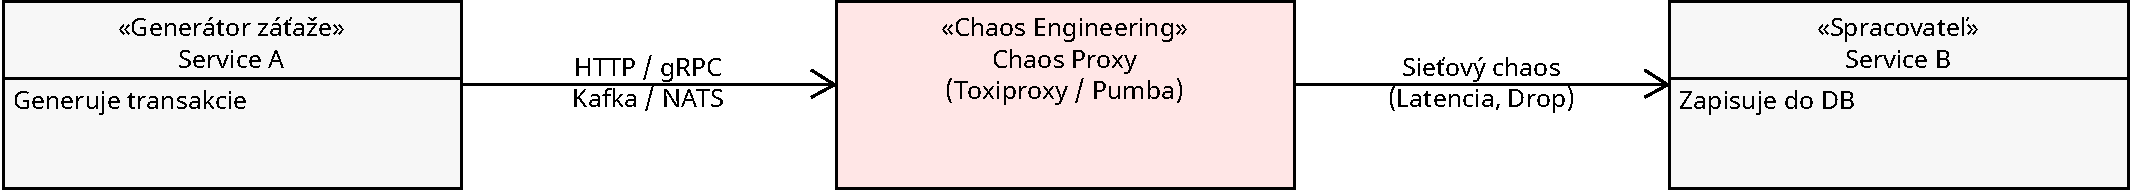
\includegraphics[width=0.8\textwidth]{architektura-crop.pdf}
\caption{Architektúra testovacieho stojanu a injekcia sieťových chýb.}
\label{f:architektura}
\end{figure}

Ako môžeme vidieť na obrázku~\ref{f:architektura}, všetka komunikácia medzi generátorom a spracovateľom prebieha cez prostredníka, ktorý simuluje sieťovú degradáciu.

\section{Porovnanie komunikačných technológií} \label{s: protokoly}

V rámci experimentov sa porovnávajú štyri kľúčové komunikačné prístupy rozdelené do dvoch kategórií:

\subsection{Synchrónna komunikácia} \label{s: synchro}
\begin{itemize}
\item \textbf{HTTP/REST (JSON):} Štandardné textové rozhranie. Výhodou je jednoduchá čitateľnosť, nevýhodou vyšší objem prenášaných dát a náročnejšia serializácia.
\item \textbf{gRPC (Protobuf):} Výkonný RPC rámec využívajúci binárny formát. Poskytuje nízke nároky na sieťové pásmo a podporuje obojsmerné streamovanie~\cite{Indrasiri2020}.
\end{itemize}

\subsection{Asynchrónna komunikácia} \label{s: asynchro}
\begin{itemize}
\item \textbf{Apache Kafka:} Distribuovaná platforma pre spracovanie udalostí s vysokou priepustnosťou a trvalým ukladaním správ na disk.
\item \textbf{NATS JetStream:} Ľahkovedný a extrémne rýchly messaging systém zameraný na nízku latenciu a jednoduchú správu.
\end{itemize}

\section{Vyhodnotenie vzorov odolnosti (Resilience Patterns)} \label{s: vzory}

Na zamedzenie kaskádových zlyhaní pri sieťových degradáciách boli do komunikácie integrované tri kľúčové vzory~\cite{Richardson2018}:

\paragraph{Retries s exponenciálnym odstupom (Exponential Backoff).}
Zabezpečuje opakované odoslanie zlyhanej požiadavky s postupne sa zvyšujúcim časovým intervalom, čím sa predchádza zahusteniu siete.

\paragraph{Circuit Breaker.}
Monitoruje chybovosť cieľového servisu. Ak podiel chýb prekročí definovaný prah, preruší odosielanie požiadaviek, čím dáva zlyhávajúcemu servisu čas na zotavenie~\cite{Montesi2016}.

\paragraph{Rate Limiting.}
Obmedzuje maximálny počet spracovaných požiadaviek za sekundu (RPS) na vstupe do servisu, čím chráni systém pred preťažením.

\subsection{Merané metriky} \label{s: metriky}
Sledovanie výkonnosti prebieha pomocou Prometheus a vizualizácie v Grafana. Hodnotia sa nasledujúce parametre:
\begin{itemize}
\item \textbf{Priepustnosť (Throughput):} Počet úspešne spracovaných požiadaviek za sekundu (RPS).
\item \textbf{Latencia (P95 / P99 Latency):} Čas odozvy pre najpomalších $5\,\%$ a $1\,\%$ požiadaviek~\cite{Dean2013}.
\item \textbf{Miera chybovosti (Error Rate):} Percentuálny podiel zlyhaných transakcií.
\item \textbf{Čas obnovy (Recovery Time):} Čas potrebný na návrat do normálneho stavu po odstránení sieťovej poruchy.
\end{itemize}

\section{Záver} \label{s: zaver}

Výstupom tohto semestrálneho projektu bude ucelená inžinierska analýza a rozhodovacia matica (Trade-off Matrix). Výsledky poskytnú praktické odporúčania pre výber vhodného komunikačného protokolu a nastavenie vzorov odolnosti v závislosti od požiadaviek na latenciu, priepustnosť a toleranciu voči sieťovým výpadkom v reálnych produkčných systémoch.

\bibliography{literatura}
\bibliographystyle{plain}

\end{document}